% ****** Start of file aipsamp.tex ******
%
%   This file is part of the AIP files in the AIP distribution for REVTeX 4.
%   Version 4.1 of REVTeX, October 2009
%
%   Copyright (c) 2009 American Institute of Physics.
%
%   See the AIP README file for restrictions and more information.
%
% TeX'ing this file requires that you have AMS-LaTeX 2.0 installed
% as well as the rest of the prerequisites for REVTeX 4.1
%
% It also requires running BibTeX. The commands are as follows:
%
%  1)  latex  aipsamp
%  2)  bibtex aipsamp
%  3)  latex  aipsamp
%  4)  latex  aipsamp
%
% Use this file as a source of example code for your aip document.
% Use the file aiptemplate.tex as a template for your document.
\documentclass[
aip,
%jmp,%
%bmf,%
%sd,%
rsi,%
amsmath,amssymb,
%preprint,%
reprint,%
%author-year,%
%author-numerical,%
]{revtex4-1}

\usepackage{graphicx}% Include figure files
\usepackage{dcolumn}% Align table columns on decimal point
\usepackage{bm}% bold math
%\usepackage[mathlines]{lineno}% Enable numbering of text and display math
%\linenumbers\relax % Commence numbering lines

\newcommand	 {\sbar}	{{s}}
\newcommand	 {\rbar}	{{r}}
\newcommand	 {\hi}		{{h_\mathrm{i}}}
\newcommand	 {\pii}  	{{p_\mathrm{i}}}
\newcommand	 {\kb}		{{k_\mathrm{B}}}
\newcommand	 {\Tlow}	{{T_\mathrm{low}}}
\newcommand 	 {\Pnat} 	{{P_\mathrm{nat}}}
\newcommand {\QIA}	{{Q_\mathrm{IA}}}
\newcommand {\QIB}	{{Q_\mathrm{IB}}}
\newcommand {\QIIA}	{{Q_\mathrm{IIA}}}
\newcommand {\QIIB}	{{Q_\mathrm{IIB}}}
\newcommand {\Pcut}     	{{P_\mathrm{cut}}}
\newcommand {\TlowI}     {{T^\mathrm{I}_\mathrm{low}}}
\newcommand {\TlowII}    {{T^\mathrm{II}_\mathrm{low}}}
\newcommand {\Ptot}	{{P_\mathrm{tot}}}
\newcommand {\PIA}    	{{P_\mathrm{IA}}}
\newcommand {\PIB}    	{{P_\mathrm{IB}}}
\newcommand {\PIIA}    	{{P_\mathrm{IIA}}}
\newcommand {\PIIB}    	{{P_\mathrm{IIB}}}
\newcommand {\Eave}	{{E_\mathrm{ave}}}
\newcommand {\sigE}	{{\sigma_{\left < E \right >}}}
\newcommand {\SR}		{${\mathrm{S16}_{144}}$}
\newcommand {\SI}		{${\mathrm{S16}_{1024}}$}	
\newcommand {\SII}		{${\mathrm{S35}_{1024}}$}

\begin{document}

\preprint{AIP/123-QED}

\title[Multisequence Monte Carlo simulations]{Multisequence algorithm for coarse-grained biomolecular simulations: exploring the sequence-structure relationship of proteins}

\author{A. Aina}
\author{S. Wallin}
\email{swallin@mun.ca}
\affiliation{ 
Memorial University of Newfoundland, Department of Physics and Physical Oceanography, A1B 3X7 St John's, NL, Canada}

\date{\today}

\begin{abstract}
We consider a generalized-ensemble algorithm for coarse-grained simulations of biomolecules which allows the thermodynamic behavior of two or more sequences to be determined in a single ``multisequence" run. By carrying out a random walk in sequence space, the method also enhances conformational sampling. Escape from local energy minima is accelerated by visiting sequences for which the minima are more shallow or absent. We apply the method alongside an intermediate-resolution coarse-grained model for protein folding with 7 atoms per amino acid and 3 amino acid types. The potential for large-scale coverage of sequence space is explored by applying the method to two sets with $>$1,000 sequences each. The resulting thermodynamic data is used to explore the sequence-structure and sequence-stability relationships between pairs of protein folds with different secondary structures.
\end{abstract}

\pacs{87.14.E; 87.15.A; 05.10.Ln}
                             
\keywords{Monte Carlo, generalized ensembles, protein folding, protein fold switching}

\maketitle

\section{Introduction}
\noindent
Recent years have seen important advances in biomolecular simulation methods, including improvements to standard molecular dynamics force fields,~\cite{Piana2014} the advent of several alternative atomistic simulation approaches,~\cite{Ding2008,Irback2006,Verma2009,Yang2007} and new techniques for  conformational sampling.~\cite{Bernardi2015} Together with the ever-increasing availability of computational resources, these advances have triggered a few major efforts~\cite{McGuffee2010,Miao2010,Perilla2016,Lindorff-Larsen2011,Yu2016} to characterize the dynamics of biomolecular systems of various sizes, e.g., a small native protein on the millisecond scale~\cite{Lindorff-Larsen2011} and a comprehensive model cytoplasm on the nanosecond scale.~\cite{Yu2016} While encouraging and insightful, these large-scale simulations have also highlighted the fact that severe tradeoffs in size and time scales will likely persist for the foreseeable future. 

One way to expand the range of biomolecular simulations is to turn to coarse-grained (CG) models, where the basic aim is to simplify the physical description of interactions while retaining the essential physics of the system under study.~\cite{Riniker2012} Ingolfsson \textit{et al.} list 4 main factors that make CG models computationally fast: reduction in the number of degrees of freedom, faster simulation dynamics, emphasis on short-range interactions and the ability of using larger integration time steps.~\cite{Ingolfsson2014} To this list can be added that a CG representation of either the interaction potential or the molecular geometry often opens up for alternative sampling schemes beyond traditional molecular dynamics approaches, which can further speed up conformational sampling. Examples of such sampling schemes include activation-relaxation kinetics,~\cite{Beland2011} discrete molecular dynamics~\cite{Proctor2011} and various Monte Carlo (MC)-based techniques such as cluster moves.~\cite{Vitalis2009} 

The challenges of achieving representative conformational sampling of individual biomolecular systems notwithstanding, many biological processes naturally call for the investigation and comparison of molecular variants. This is required, for example, in determining the molecular mechanisms of specificity in protein-protein~\cite{Zarrinpar2003,Hakes2007} or protein-nucleotide interactions,~\cite{Rohs2010} and the role of mutations in disease processes such as protein aggregation.~\cite{Ross2004} Another example is the protein folding process, where unique insight has been achieved by comparing the folding within and between protein families.~\cite{Tzul2017,Wensley2010} In a situation with rapid growth of sequence information,~\cite{Vukmirovic2000} it is of interest to explore ways to efficiently sample multiple sequences in biomolecular simulations. 

To this end, we consider in this work an MC-based algorithm that can calculate the thermodynamics of multiple sequences in a single run and apply it to a coarse-grained model for protein folding. This multisequence (MS) method was originally developed in the context of homo- and heteropolymer simulations~\cite{Irback1995} and was also later adapted for the characterization of peptide-protein binding specificity.~\cite{Bhattacherjee2013,Wallin2017} To our knowledge, however, it has not been previously tested in realistic protein folding simulations. The MS algorithm carries out a simulation in a generalized ensemble that performs a random walk in sequence space. Hence, there are two main types of updates: conformational updates $\rbar\rightarrow\rbar'$ and sequence updates $\sbar\rightarrow\sbar'$. As illustrated in Fig.~1, this strategy can be applied when $\rbar$ and $\sbar$ are ``perpendicular" coordinates such that the potential energy of the model can be written in terms of two independent variables, $E(\sbar,\rbar)$. While this may be hard to achieve for detailed biomolecular models, it is likely possible in many CG models.

As an initial test case, we apply the MS method to a set of 144 model protein sequences with 16 amino acids. This set (denoted here {\SR}) was constructed to sparsely cover the sequence space between two ideally designed sequences, A1 and N1, which fold into an $\alpha$-helix and a $\beta$-hairpin, respectively.~\cite{Bhattacherjee2012} In a previous work, this set allowed us to demonstrate the existence of A1-N1 mutational pathways which do not proceed through disordered (non-folding) sequences but instead switch abruptly between the two folds in a single mutational step.~\cite{Holzgrafe2014} Moreover, it allowed the exploration of the biophysical factors that underpin this ``fold switching" phenomenon,~\cite{Holzgrafe2015} which was recently demonstrated in a handful of natural and engineered proteins.~\cite{Bryan2010} Here we use the set {\SR} and our CG model for protein folding to validate the MS method and compare its efficiency to a standard generalized-ensemble method.~\cite{Marinari1992,Lyubartsev1992} We thereafter greatly enlarge {\SR} to a set with 1,024 sequences, also spanning the A1-N1 space, as well as another set of the same size spanning two 35-amino acid sequences, A2 and TN, that fold into two-helical bundle and mixed $\alpha$-$\beta$ structures, respectively. Besides showing that the MS method can be applied to large numbers of sequences, the results allow us to carry out a more systematic analysis of the biophysical character of sequences along mutational pathways connecting these two pairs of basic folds than has been previously possible. 

\begin{figure}
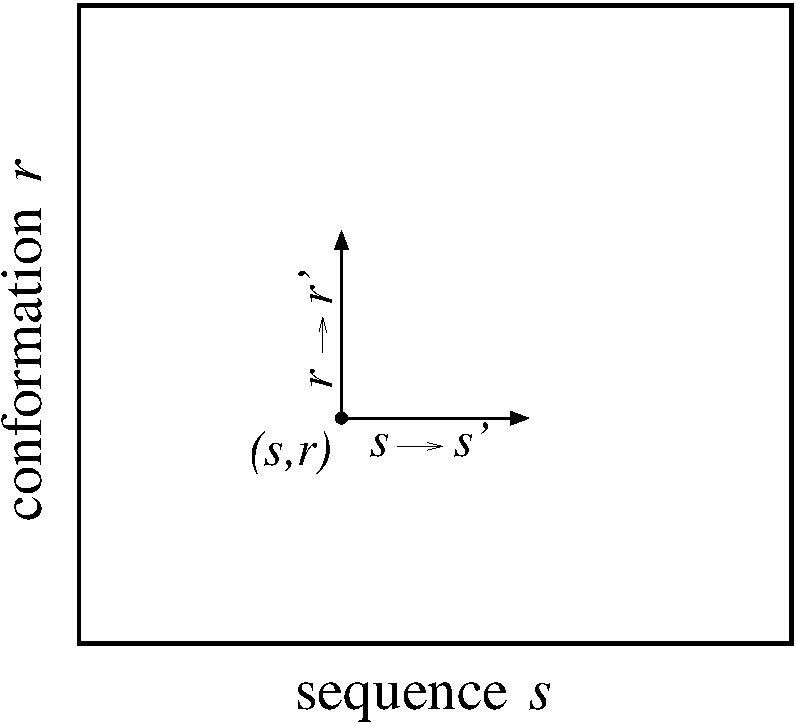
\includegraphics[width=4.2cm]{Fig1}
\caption{The two types of Monte Carlo updates in the multisequence Monte Carlo algorithm.}
\end{figure}

\section{Theory}

\subsection{Generalized-ensemble algorithms and simulated tempering}
\noindent
Conventional Monte Carlo simulations of the canonical distribution is problematic at low temperatures $T$ for many physical systems because simulations tend to become trapped in local energy minima and hamper representative sampling of configurational space. The basic idea of generalized-ensemble algorithms~\cite{Mitsutake2001} is to alleviate this trapping problem by sampling states using a non-Boltzmann weight factor and/or expand the state space with additional dynamical parameters, such that a more efficient random walk in potential energy can be achieved. 

A well-known generalized-ensemble algorithm is simulated tempering (ST),~\cite{Marinari1992,Lyubartsev1992} in which it is the temperature $T$ that becomes a dynamic parameter. In this scheme, frequent visits to high-$T$ allow simulations to readily escape from local energy traps. The ST algorithm thus simulates the joint probability distribution 
\begin{equation}
P(\rbar,m) =\dfrac{1}{\hat{Z}} e^{-\beta_m E(\rbar) + g_m}\,,
\label{ST}
\end{equation}
where  $\beta_m=1/k_\mathrm{B} T_m$, $\{T_m\}_{m=1}^\mathrm{M}$ a set of temperatures and $k_\mathrm{B}$ is Boltzmann's constant. The normalization constant in Eq.~\ref{ST} is  
\begin{equation}
\hat{Z} = \sum_r \sum_{m=1}^{\mathrm{M}}e^{-\beta_m E(\rbar) + g_m}\,,
\end{equation}
where the first sum is over all conformations $\rbar$. The simulation parameters $g_m$ control the marginal probability distribution
\begin{equation}
P(m) = \frac{1}{\hat{Z}}\sum_r e^{-\beta_m E(\rbar) + g_m} \,,
\end{equation}
and must therefore be carefully chosen. A common and convenient choice is $g_m\approx \beta_m F_m$, where $F_m$ is the free energy at temperature $T_m$. With this choice, $P(m)$ becomes approximately flat ensuring all temperatures are frequently visited. 

\subsection{Multisequence algorithm}
\noindent 
The basic idea of the MS algorithm for biomolecular simulation is to let the sequence $\sbar$ become a dynamic parameter rather than the temperature as in ST. A dynamic $\sbar$ is technically feasible as long as the potential energy can be written as $E(\sbar,\rbar)$, where $\sbar$ and $\rbar$ are independent variables. This is the case in our coarse-grained protein model with only backbone degrees of freedom and can also be achieved for more detailed  models~\cite{Bhattacherjee2013,Wallin2017}. 

In analogy with ST, the MS algorithm simulates the joint probability distribution
\begin{equation}
P(\sbar,\rbar) =\dfrac{1}{\tilde{Z}}e^{-\beta E(\sbar,\rbar) + h(\sbar)}\,, 
\label{MS}
\end{equation}
where  
\begin{equation}
\tilde{Z} = \sum_{\sbar}\sum_{\rbar} e^{-\beta E(\sbar,\rbar)+ h(\sbar)}\,
\end{equation}
and the first sum goes over a set of allowed sequences $\sbar$. The simulation parameters $h(\sbar)$, similar to the parameters $g_m$ in ST, control the marginal distribution $P(\sbar)=\tilde{Z}^{-1}\sum_{\rbar} e^{-\beta E(\sbar,\rbar)+ h(\sbar)} = \tilde{Z}^{-1}e^{-\beta F(\sbar)+ h(\sbar)}$ and a roughly flat $P(\sbar)$ can be achieved by choosing $h(\sbar) \approx \beta F(\sbar)$, where $F(\sbar)$ is the free energy of sequence $\sbar$ at temperature $T$. 

Two types of MC updates are required to sample from the distrubution in Eq.~\ref{MS}, ordinary conformational update $\rbar\rightarrow\rbar'$ and mutational updates $\sbar\rightarrow\sbar'$. The acceptance probabilities for the latter  becomes
\begin{equation}
P_\mathrm{acc} (\sbar\rightarrow\sbar') = \min [1, \exp\{-\beta\Delta E+\Delta h\}]\,,
\label{accrej}
\end{equation}
where $\Delta E = E(\sbar',\rbar)-E(\sbar,\rbar)$ and $\Delta h = h({\sbar'})-h(\sbar)$.

\section{Model and Methods}
\subsection{Coarse-grained 3-letter model for protein folding}
\noindent
All calculations were carried out using the coarse-grained model for protein folding developed in Ref.~\citenum{Bhattacherjee2012}. In this model, there are 3 different amino acid types: hydrophobic (h), polar (p) and turn-type (t). The backbone chain is represented atomistically by the N, H, $\mathrm{C}_\alpha$, $\mathrm{H}_{\alpha 1}$, C$'$ and O atoms. By contrast, the sidechain represention is simplified to a single enlarged $\mathrm{C}_\beta$ atom, which is geometrically identical for h and p types. The sidechain is absent for the t type which instead has an $\mathrm{H}_{\alpha 2}$ atom. The t type is therefore closely related to glycine. All bond lengths, bond angles, and peptide plane angles (180$^\circ$) are held fixed. Hence, an $N$-amino acid chain conformation $\rbar$ can, for any sequence $\sbar$, therefore be described by the set of 2$N$ backbone torsional angles $\{\phi_i$, $\psi_i\}_{i=1}^{N}$. 
 
This geometrical description is paired with a simplified but finely tuned energy function with 4 terms: $E= E_\mathrm{ev} + E_\mathrm{loc} + E_\mathrm{hb} + E_\mathrm{hp}$. The first two, $E_\mathrm{ev}$ and $E_\mathrm{loc}$, represent excluded-volume effects of all atoms and local electrostatic effects, respectively. The hydrogen-bond energy, $E_\mathrm{hb}$, represents directionally dependent interactions between NH and CO groups which are necessary for secondary structure formation. Finally, the ``hydrophobicity" term, $E_\mathrm{hp}$, implements pairwise Lennard-Jones-like interactions between the $C_\beta$ atoms of h amino acids which are necessary for driving chain collapse during folding. Various model parameters, e.g., the strengths of hydrophobic attractions and hydrogen bonding, were determined based on the ability of the model to spontaneously fold a set of model sequences with 18-54 amino acids into  structurally diverse and thermodynamically stable native states with both $\beta$ and $\alpha$-structure. As it turned out, this strategy made the model robust enough to fold sequences designed to have mixed $\alpha$ and $\beta$ structures. 

\subsection{Model sequences}
\noindent
Six of the model sequences studied in this work, A1, N1, R1, R2, A2, and TN, are given in Table~I. In addition, we study two sequence sets $\mathrm{S16}_{1024}$  and $\mathrm{S35}_{1024}$ with 1,024 sequences each derived from the A1-N1 and A2-TN pairs, respectively, through mutational combinations, as well as the set $\mathrm{S16}_{144}$ taken from  Ref.~\protect\citenum{Holzgrafe2014}. 
 
\begin{table}
\caption{\label{tab1} List of 6 model sequences of different lengths $N$ studied in this work.}
\begin{ruledtabular}
\begin{tabular}{lcr}
Name & $N$ & Sequence \\
\hline
A1 & 16 & pphpphhpphpphhpp \\
N1 & 16 & phphphpttphphphp \\
R1 & 16 & pphhphptthpphhpp\\
R2 & 16 & ppphphhtthhphppp\\
A2 & 35 & (A1)ttt(A1)\\
TN & 35 & (A1)ttt(N1)\\
\end{tabular}
\end{ruledtabular}
\end{table}


\subsection{Monte Carlo simulation parameters}
\noindent
Both ST and MS simulations are carried out with two types of conformational updates $\rbar\rightarrow\rbar'$: (1) a global pivot move (20\%) which randomly picks a $\phi_\mathrm{i}$ angle or $\psi_\mathrm{i}$ angle and assign a new value between $-\pi$ and $\pi$; and (2) a semi-local move (80\%) which turns the $\phi_\mathrm{i}$ and $\psi_\mathrm{i}$-angles of 4 consecutive amino acids in a coordinated manner.~\cite{Favrin2001} In MS simulations, sequence updates $\sbar\rightarrow\sbar'$ are carried out by randomly picking a new sequence $\sbar'\ne\sbar$ and applying the accept-reject criterion in Eq.~\ref{accrej}. A sequence move is attempted every $1,000$ MC steps while temperature updates $m\rightarrow m'$ are attempted every 100 steps. The simulations carried out in this work are summarized in Table~II.

\begin{table}
\caption{\label{tab2} List of simulations carried out in this work. }
\begin{ruledtabular}
\begin{tabular}{lcccr}
Runs & Algorithm & $\kb T$  & MC steps/run\footnote{Excludes a thermalization step with $10^6$ MC steps/run.} &  Sequences\\
\hline
32 & ST & 0.43--0.65 & $1\times10^7$ &A1\\ 
32 & ST & 0.43--0.65 & $1\times10^7$ &N1\\ 
32 & ST & 0.43--0.65 & $1\times10^7$ &R1\\ 
32 & ST & 0.43--0.65 & $1\times10^7$ &R2\\ 
32$\times$8\footnote{32 runs per temperature at 8 different temperatures.} & MS &0.43--0.65& $18\times 10^7$ & $\mathrm{S16}_{144}$\\
16 & MS & 0.43  & $5\times 10^9$ &  $\mathrm{S16}_{1024}$ \\
16 & MS & 0.46 & $4\times 10^9$ &  $\mathrm{S35}_{1024}$ \\
\end{tabular}
\end{ruledtabular}
\end{table}

\subsection{Observables}
\noindent
Fold stabilities are calculated as in Ref.~\citenum{Holzgrafe2015} and described briefly below. First we define two structural similarity measures $\QIA$ and $\QIB$ for folds IA and IB, respectively, indicating the fraction of the fold-specific backbone-backbone hydrogen bonds that have been formed. The fold IA-hydrogen bonds are (2,6), (3,7), (4,8), (5,9), (6,10), (7,11), (8,12), (9,13), (10,14), (11,15) and the fold IB-bonds are (3,14), (5,12), (7,10), (10,7), (12,5), (14,3), where (i,j) indicates a hydrogen bond between the CO group of amino acid i and the NH group of amino acid j. The  stabilities of folds IA and IB are then defined as the probabilities $\PIA = P(\QIA\ge0.8)$ and $\PIB = P(\QIB\ge0.80)$, respectively, i.e., the probability that at least 80\% of the fold's hydrogen bonds are formed. $\PIA$ and $\PIB$ thus depend on both sequence $\sbar$ and temperature $T$. For example, $\PIA=0.875\pm 0.003$ for A1 and $\PIB=0.785\pm0.008$ for N1 at $\kb T = 0.43$. Structural similarity measures for 35-amino acid folds IIA and IIB are defined as $\QIIA = ( Q_\mathrm{IA}^\mathrm{1-16} + Q_\mathrm{IA}^\mathrm{20-35} + Q_\mathrm{tert} ) / 3$ and $\QIIB = ( Q_\mathrm{IA}^\mathrm{1-16} + Q_\mathrm{IB}^\mathrm{20-35} + Q_\mathrm{tert} ) / 3$, respectively, where superscripts on $\QIA$ and $\QIB$ indicate over which amino acid positions those measures are applied to within the longer 35 amino acid sequences and $Q_\mathrm{tert}$ is a measure that counts the number of $\mathrm{C}_\beta$-$\mathrm{C}_\beta$ contacts between the two secondary structure elements of these folds.~\cite{Holzgrafe2015} In analogy with $\PIA$ and $\PIB$, we define the stabilities of folds IIA and IIB as $\PIIA = P(\QIIA\ge0.8)$ and $\PIIB = P(\QIIB\ge0.80)$, respectively. The root-mean-square-deviation, RMSD, is calculated over all $\mathrm{C}_\alpha$ atoms.

\begin{figure}
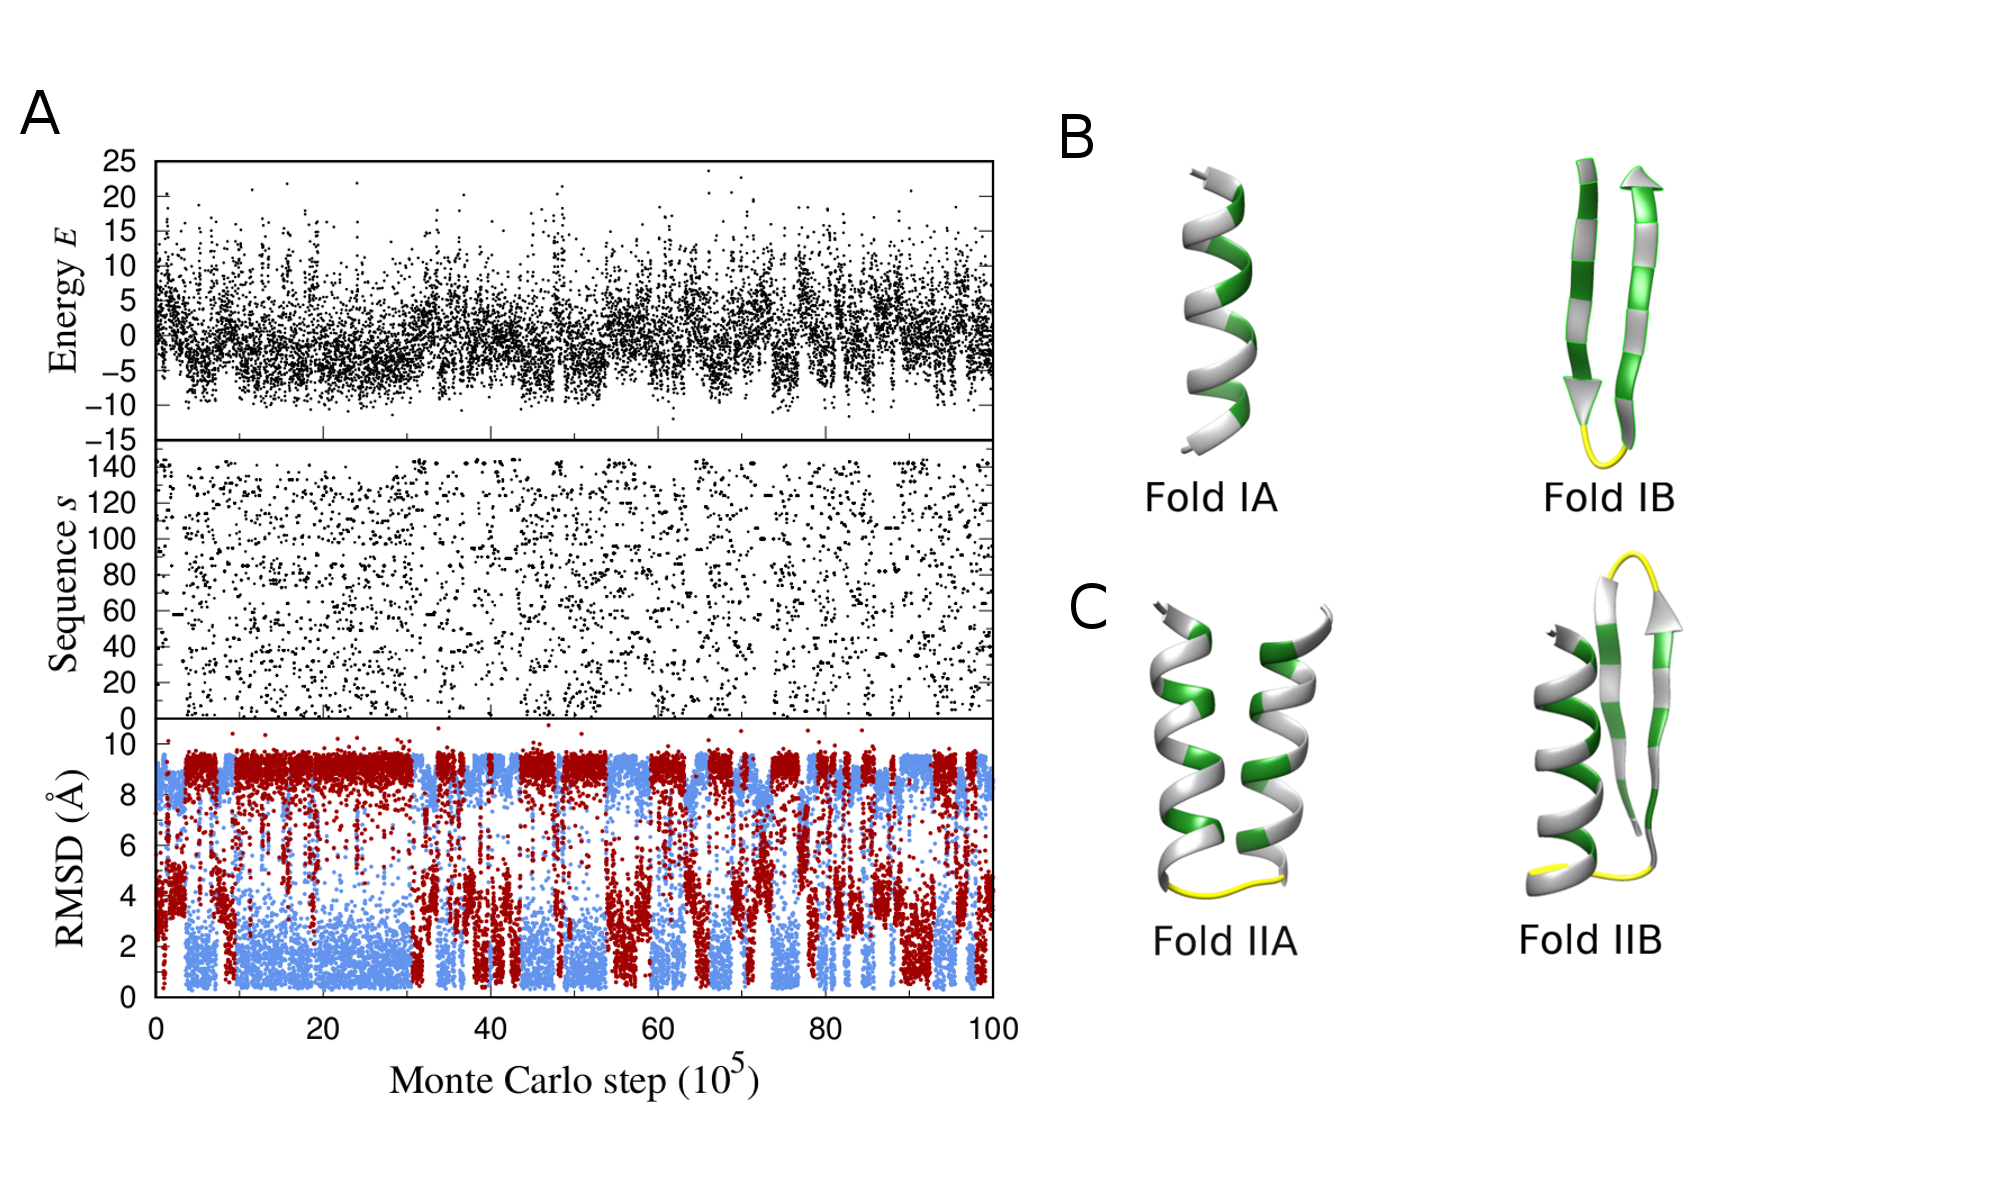
\includegraphics[width=10.0cm]{MCTrajFolds}
\caption{(A) Example of an MS simulation applied to the sequence set $\mathrm{S16}_{144}$. The plot shows the MC evolution of the sequence $\sbar$ (numbered 1--144), the total potential energy $E$ and the root-mean-square deviation (RMSD) calculated against fold IA (light blue) and fold IB (dark red) structures shown in (B). The simulation is carried out at $\kb T = 0.43$. (B) Representative structures of fold IA and fold IB, selected to be the minimum-energy conformations found for the sequences A1 and N1, respectively. (C) Representative fold IIA and fold IIB structures selected to be the minimum-energy conformations of A2 and TN, respectively. }
\end{figure}

\section{Results}

\subsection{Computational efficiency}
\noindent
We start by applying the MS algorithm to the set {\SR} across a range of temperatures $T$ (see Table~II). Two of the sequences in {\SR} are A1 and N1 (see Table~I) which fold into stable $\alpha$-helix and $\beta$-hairpin structures, respectively, as shown in Fig.~2B. A1 and N1 differ at 10 positions such that 10 consecutive point mutations can transform A1 into N1, and vice versa. The binary sequence space between A1 and N1 in which any combination of these mutations have been carried out, therefore contains $2^{10}=1,024$ sequences. The 144 sequences in {\SR} were selected from this binary space with the constraints that the total number of hydrophobic amino acids are not too high and that they are not too unevenly distributed.~\cite{Holzgrafe2014}

\begin{figure}
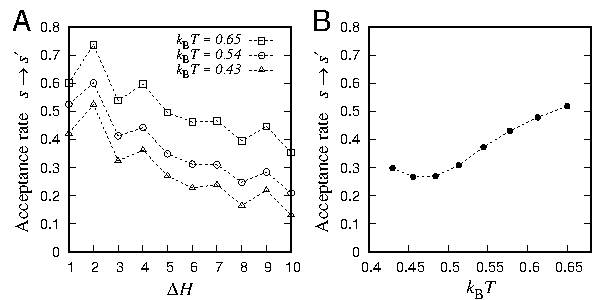
\includegraphics[width=7.8cm]{Pacc}
\caption{Acceptance rates for $\sbar\rightarrow\sbar'$ updates in MS simulations of the {\SR} sequence set as a function of (A) the number of changed amino acid positions $\Delta h$ and (B) temperature $T$. Acceptance rates for 3 different $T$'s are shown in (A).}
\end{figure}

Figure~2 illustrates a typical MS simulation trajectory carried out at the lowest studied temperature which is below the folding temperature of both A1 and N1.~\cite{Holzgrafe2014,Holzgrafe2015} From the MC evolution of the total energy $E$, sequence index $\sbar$, and RMSD values from the representative structures in Fig.~2B, it is evident that visits to various sequences drive transitions into a range of structural states. In particular, there are frequent visits to both $\alpha$-helix and $\beta$-hairpin structures and transitions between them are accompanied by a shift in which sequences are preferably visited. For example, visits to high $\sbar$-indices, including N1 with index 144, tend to coincide with formation of $\beta$-hairpin structures as required to generate the correct equilibrium conformational ensembles. 

One might have suspected that the MS algorithm would be hampered by poor acceptance rates for sequence updates. However, this is not the case in our model. We carry out updates $\sbar\rightarrow\sbar'$ by picking a new random sequence $\sbar'\ne\sbar$ from the set of allowed sequences. The (average) acceptance rate  depends on both $T$ and the step in sequences space $\Delta h$, i.e., the number of amino acid positions changed, as shown in Fig.~3. At the lowest $T$ and highest $\Delta h$, acceptance rates are only around 0.1-0.2. However, for most other $T$ and $\Delta h$ the overall acceptance rate is substantially higher and often above the oft-quoted rule-of-thumb value 0.25~\cite{Gilks1996} (see Fig~4B). We note therefore that increased acceptance rates can easily be achieved by restricting proposed updates such that $\Delta h\le\Delta h_\mathrm{max}$, where $\Delta h_\mathrm{max}$ is a maximum step size, which might be necessary for longer chains. 

\begin{figure}
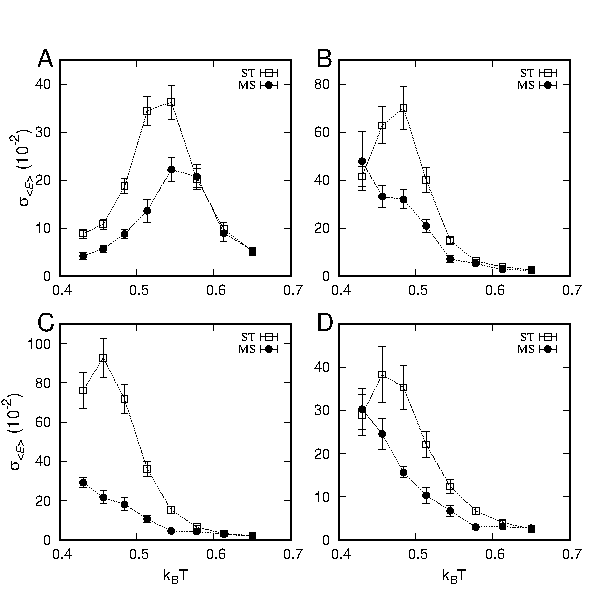
\includegraphics[width=8.0cm]{Stderr}
\caption{Comparing sampling efficiency of the MS and ST algorithms. Statistical errors $\sigma_{\left < E\right >}$ of the average total energy $\left < E\right >$ from the two methods for the 16-amino acid sequences (A) A1, (B) N1, (C) R1 and (D) R2. Simulation lengths in the two methods are adjusted such that the number of conformations sampled per sequence and temperature is roughly the same (see text). }
\end{figure}

We now compare the results from our MS calculations with simulated tempering (ST) simulations carried out on 4 of the 144 sequences, namely A1 and N1 and two random sequences, R1 and R2, chosen at distances $h=4$ and $h=6$ from A1, respectively (see Table~I). While ST provides the thermodynamics of a given sequence across a range of $T$ in a single run, an MS simulation provides the thermodynamics of all 144 sequences at one $T$. We adjust the simulation lengths for ST and MS runs such that roughly the same number of sampled conformations are obtained for each $\sbar$ and $T$ combination, thus ensuring that similar computational resources are used for the two algorithms (see Table~II). We first validate the MS algorithm by comparing the average total energy, $\left < E \right >$, calculated for these 4 sequences with the two different methods (see Supplementary Information). The two sets of results are entirely consistent showing that, for a given $\sbar$ and $T$, both MS and ST indeed sample the same distribution. 

As a way to assess conformational sampling efficiency, we compare in Fig.~4 the statistical error, $\sigE$, of the average energy $\left <E\right >$ for the 4 sequences obtained using ST and MS, respectively. Because approximately the same number of sampled conformations were obtained for each combination of $\sbar$ and $T$, we compare the statistical errors directly. At the highest studied $T$, which is well above the folding temperature of both A1 and N1, the two algorithms give almost identical statistical errors. This can be understood by noting that at high-$T$ the free-energy landscape is relatively smooth and conformational space requires little difficulty to sample. The benefit of adding a dynamic parameter, whether $\sbar$ or $T$, is apparently minor under these conditions. However, at lower $T$, the $\sigE$ values from MS is often smaller than those from ST and never significantly higher. For example, at the lowest $T$, the precision in the estimate of $\left < E\right >$ is roughly twice as high in MS than ST for A1 and R1, and roughly the same for N1 and R2. 

%The best estimate occurs at $\kb\approx$ 0.46 where MS is about 450\% better than ST. Even at the lowest T studied, MS is at least consistent or better than ST for all 4 sequences.


\begin{figure*}
\rotatebox{0}{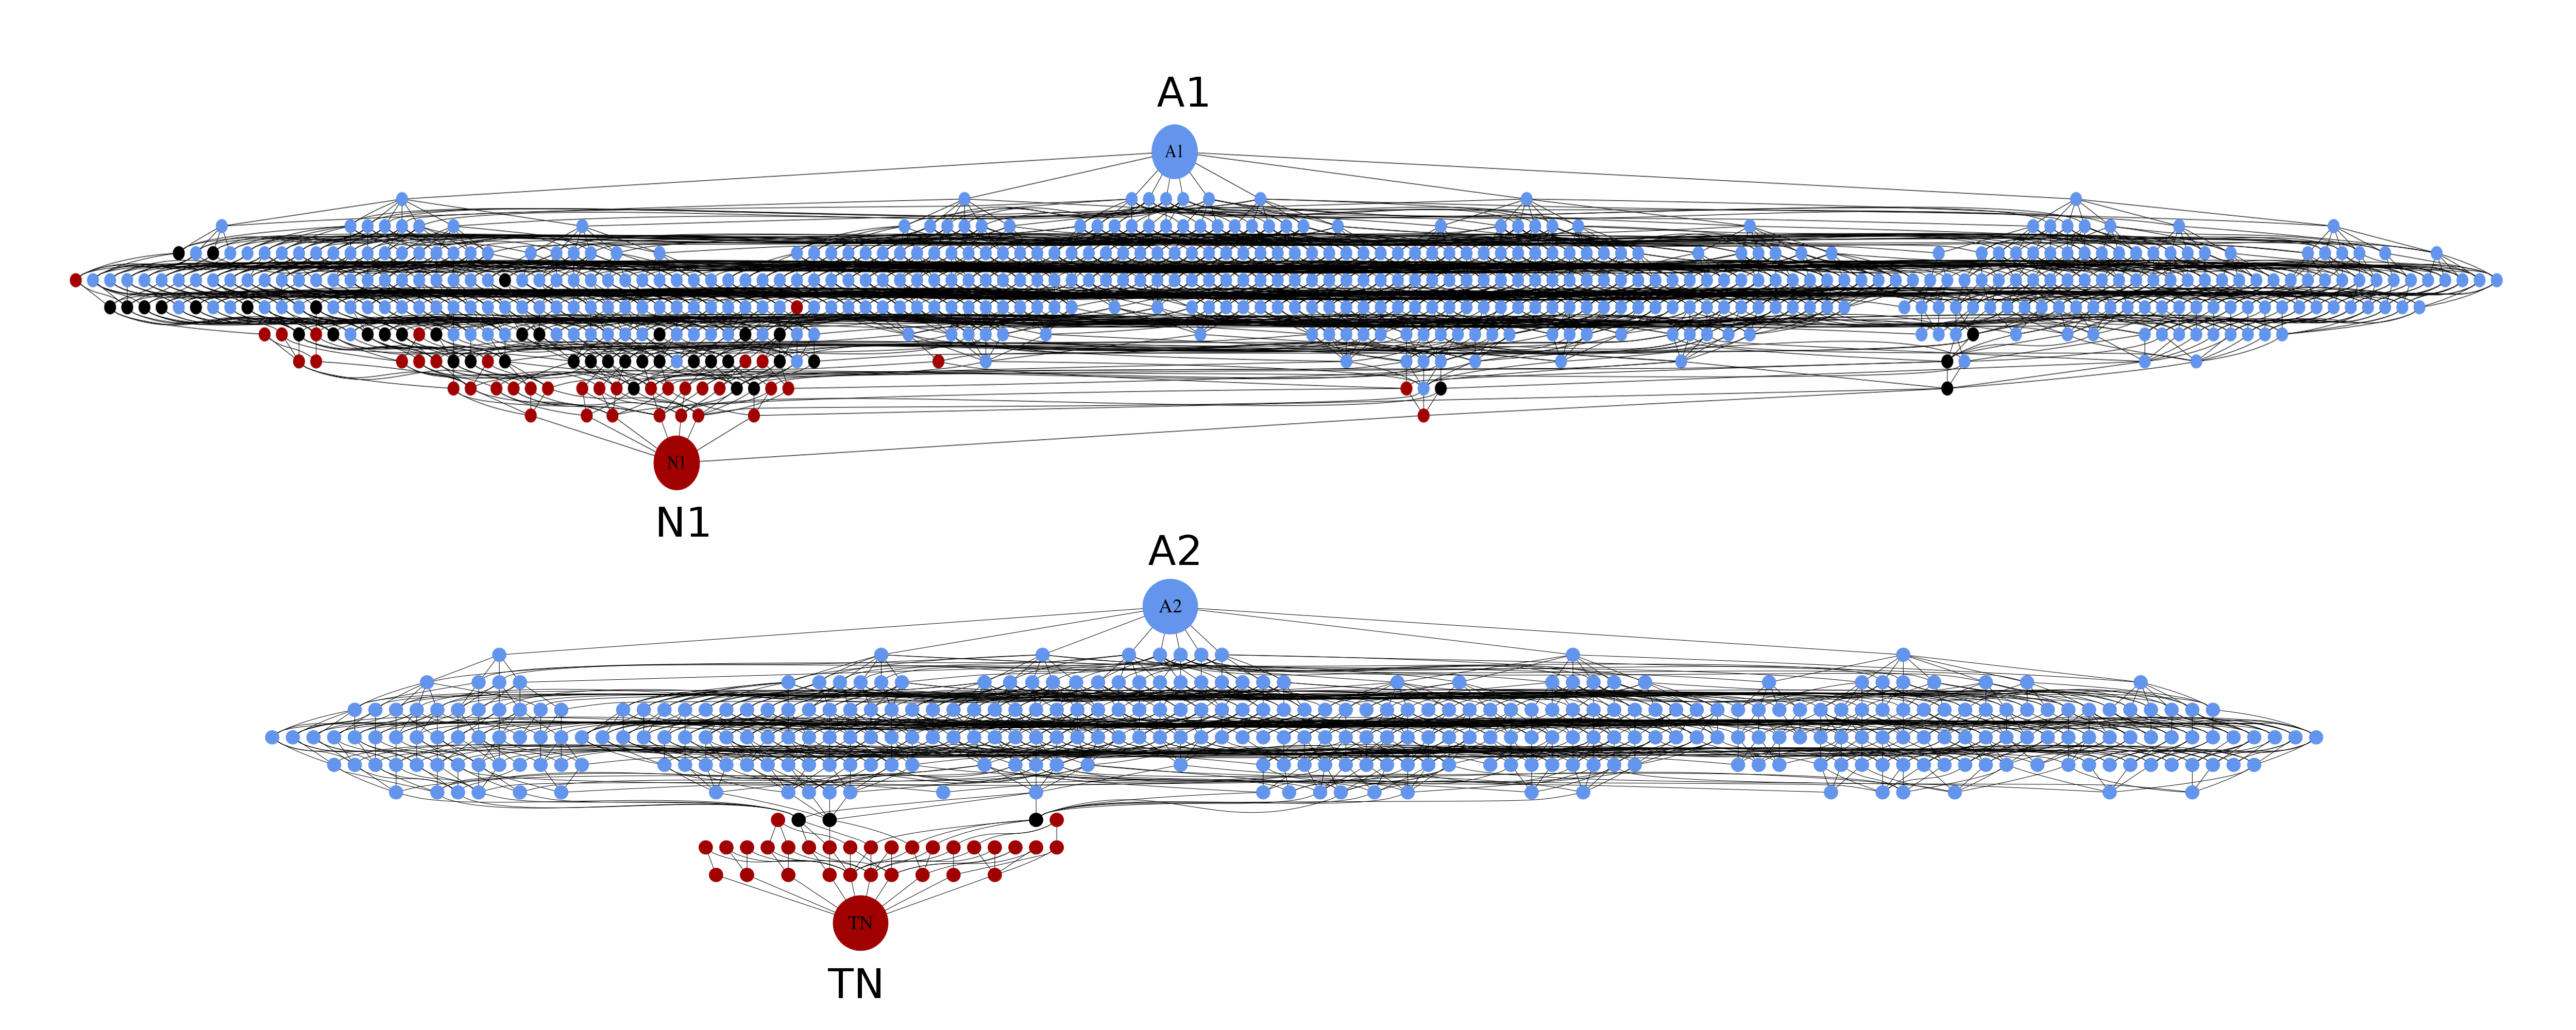
\includegraphics[width=16.6cm]{network}}
\caption{Networks of sequences connecting folds IA and IB (top) and folds IIA and IIB (bottom). Each node represents a stable sequence ($\Ptot\ge\Pcut$ where $\Pcut=0.50$) that folds into either IA or IIA (light blue), IB or IIB (dark red), or is classified as bistable ($B>0.5$, black). A line between two nodes indicates that the sequences differ at only one position. Graph created using the tool Graphviz~\protect\cite{Graphviz2000} obtained from  www.graphviz.org.}
\end{figure*}

\vspace{12pt}
\subsection{Exploring sequence space: IA/IB and IIA/IIB fold connectivities}
\noindent
We now turn to the full binary sequence sets {\SI} and {\SII} with 1,024 sequences each. By applying the MS method to these two sets (see Table~II), we determine the low-$T$ thermodynamic behavior of each included sequence. In particular, we calculate the stabilities of folds IA and IB, $\PIA$ and $\PIB$, for all sequences in {\SI} and the stabilities of folds IIA and IIB, $\PIIA$ and $\PIIB$, for all sequences in {\SII} (see Methods). The relative statistical errors on these quantities vary but are only a few percent at the most, despite the large number of sequences included.  

Having calculated these fold stabilities, we are in a position to determine if there are pathways in sequence space that lead to abrupt IA-IB or IIA-IIB fold changes, i.e., paths that do not pass through an unstable intermediate sequence. To this end, we construct graphs in which each stable sequence is represented by a node and any two nodes are connected if their sequences differ at a single amino acid position. To determine if a sequence is stable we use the criterion $P_\mathrm{tot}>\Pcut$, where  $\Ptot = \PIA + \PIB$ and $\PIIA + \PIIB$ for the IA-IB and IIA-IIB fold pairs, respectively; $\Ptot$ thus indicates the total stability of a sequence across the two competing folds. The precise network depends, of course, on the cut-off value of $\Pcut$ and a higher $\Pcut$ generally means a selection of more stable pathways. 

Fig.~5 illustrates the networks obtained with $\Pcut=0.50$ showing that, at this stability threshold, there are mutational pathways that connect both IA-IB and IIA-IIB. A precise analysis shows that there are 516,972 viable IA-IB paths and 57,912 viable IIA-IIB paths. Because there are $10! =3,628,800$ possible paths between start and end points in both cases, they represent 14.2 \% and 1.6 \% of all possible paths of the A1-N1 and A2-TN sequence pairs, respectively. Hence, folds IA and IB are rather highly connected in our model for $\Pcut= 0.50$. For $\Pcut=0.60$, the numbers are 104,640 paths (2.9\%) for IA-IB and 22,512 (0.6\%) paths for IIA-IIB. We find that there are no possible IA-to-IB or IIA-to-IIB paths when $\Pcut\ge0.74$ and $\ge 0.66$, respectively. \\

\subsection{Biophysical properties of fold-to-fold mutational pathways}
\noindent 
An apparently general characteristic of designed and natural proteins that exhibit mutation-induced fold switching is a reduced stability near the switch point.~\cite{Alexander2009,He2012,Kouza2012,Sikosek2016,Sutto2012} Our model proteins exhibit a similar trend. Fig.~6A and B show the average total stability $\Ptot$ for sequences found at different Hamming distances $h$ from the starting point. Intermediate sequences are less stable than sequences at distances $h=0$ (A1 or A2) and $h=10$ (N1 or TN), although there are large variations between sequences as indicated by the spread between upper and lower bounds. There is nonetheless a clear statistical trend that sequences become gradually less stable as successive mutations are applied to any of the 4 start and end points until a minimum is reached. 
%These minima in stability occur closer to N1 and TN in the two systems, respectively, indicating that the IA/IIA folds are more mutationally robust than the IB/IIB folds. 

\begin{figure}
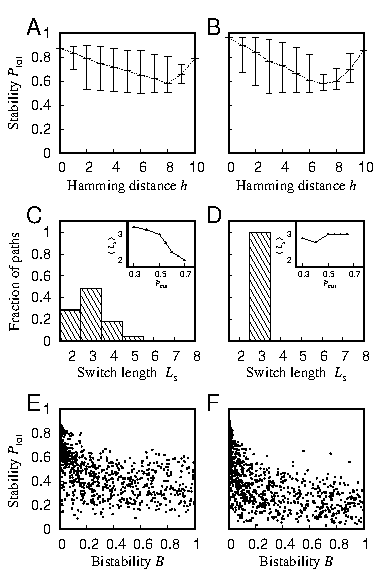
\includegraphics[width=7.8cm]{Paths}
\caption{Stability properties of mutational pathways. The total stability $\Ptot$ as a function of the distance $h$ from A1 averaged over all (A) IA-IB and (B) IIA-IIB mutational paths obtained with $\Pcut=0.50$. Error bars indicate maximum and minimum $\Ptot$ values. The distribution of switch lengths $L_\mathrm{s}$ for the (C) IA-IB and (D) IIA-IIB mutational paths ($\Pcut=0.50$). C and D insets: Average switch length $\left < L_\mathrm{s}\right >$ across all paths as a function of $\Pcut$. Scatter plots of $\Ptot$ versus bistability $B$ for all sequences in (E) {\SI} and (F) {\SII}, where $B=1-\Delta P/\Ptot$ and $\Delta P = |\PIA-\PIB|$ or $|\PIIA-\PIIB|$.}
\end{figure}

%The smooth average stability trends in Fig.~6 might have been underpinned by individual mutational pathways that gradually shift the population between the two folds, however, this is not the case.

However, the smooth stability trends in Fig.~6A and B belie the real character of the individual mutational pathways which tend to exhibit an abrupt switch between the two folds. To see this and to further examine the character of the fold transitions in our model, we make a distinction between two types of stable sequences: those that fold into a single unique fold, thus behaving as classical proteins, and those that display substantial stabilities of both folds. Such ``bistable" sequences are interesting from a biophysical perspective in that they might continuously alternate between two different folds in a highly dynamic and coordinated fashion. Indeed, bistable sequences have been proposed to play a role in the evolution of new protein folds.~\cite{Sikosek2012} We consider a stable sequence to be bistable if $B>0.5$, where $B$ is a bistability measure (see Fig.~6 legend). In principle, a fold transition can occur directly between two classical proteins with unique folds, or it can proceed via one or more intermediate bistable sequences which populate both folds. We define the switch length of a mutational pathway $L_\mathrm{s}=2+n_\mathrm{B}$, where $n_\mathrm{B}$ is the number of bistable sequences in between the two classical sequences that define the switch point. Hence, a path with $L_\mathrm{s}=2$ accomplishes a fold switch in a single mutational step without going through a bistable point. From the distributions of  $L_\mathrm{s}$ in Fig.~5C and D, taken over all pathways with $\Pcut=0.50$, it can be seen that fold switching along individual pathways are typically completed in only 1-2 mutations and a single step is often sufficient to switch between the IA and IB folds. Hence, fold switching is typically abrupt and, for $\Pcut = 0.5$, it is fairly common that viable pathways pass through one or two bistable sequences. 

Interestingly, switching between folds IA and IB through one or more bistable sequences become less and less frequent as selections for more stable pathways are made. This can be seen from the decrease in $\left <L_\mathrm{s}\right >$ as a function of $\Pcut$ (see Fig.~5C(inset)). For $\Pcut\ge0.70$, there are no longer any remaining path between the $\alpha$-helix and $\beta$-hairpin that passes through a bistable sequence because $\left <L_\mathrm{s}\right > =  2$. An underlying reason for the occurrence of sharper fold switches for more stable mutational pathways is apparent from a comparison between $\Ptot$ and $B$ across all sequences in {\SI}. As shown in Fig.~5E, sequences with the highest $\Ptot$ tend to exhibit very little bistability. Hence, highly stable paths are therefore forced to go through abrupt switch points where they transition directly between folds in a single step. The situation for the IIA-IIB fold pair is more complicated. We find that, just as for {\SI}, sequences in {\SII} follow the trend that the highest $\Ptot$ values occur for only classical, low-$B$ proteins. One might therefore expect that selection of more stable IIA-IIB paths would decrease $\left <L_\mathrm{s}\right >$, however, this is not the case as such abrupt switch points between the IIA and IIB are not available for $\Pcut\ge0.50$ (cf. Fig.~5 bottom). As a result, bistable sequences do play a crucial role in bridging the IIA and IIB folds, although passing though these sequences lead to additional reduction in stability at the switch point. 

%. Hence, passing through sequences displaying substantial bistability may still be required to mutationally drive switching between certain fold pairs as single-step transitions are not available, thereby 
 
%The sequences {\SII} do also follow this same trend (Fig.~5F). However, bistable sequences do play a crucial role in bridging the folds IIA and IIB even though their stabilities are significantly reduced, all stable mutational pathways must pass through one bistable sequences. \\

%\subsection{Super-highways in sequence space}
%
%While there are a large number possible pathways (for $\Pcut<0.60$) in both systems, there are relatively few ways to pass between the two neutral nets. For $\Pcut=0.50$, we find that there are 109 nodes in the IA neutral net and 34 nodes in the IIB neutral net through which all viable pathways pass. For $\Pcut=0.60$, these numbers reduce to 14 and 10 nodes in the IA and IIA neutral nets, respectively.
%
 
\section{Discussion}
\noindent
We have evaluated a biomolecular simulation algorithm that works by making the sequence a dynamic parameter by testing it on a CG model for protein folding. The results indicate that there are two main potential benefits of this approach. Firstly, it provides a convenient way to sample the canonical distributions of a large set of sequences in a single run and, secondly, it enhances the sampling of conformational space such that it can be applied directly at low temperatures. The conformational sampling efficiency can be assessed from the comparison with ST. Although there is no single ``fair" way to compare the MS and ST methods, we chose as a measure of efficiency the statistical error of the total energy, $\sigE$, obtained with roughly the same computational cost per temperature and sequence. At the highest studied temperatures, we find that the statistical errors $\sigE$ are basically the same for the two methods. This finding is not unexpected because conformational sampling of short polymers at high $T$ does not involve crossing any major energy barriers. As a result, successively sampled conformations for a given combination of sequence $\sbar$ and temperature $T$, are therefore likely mostly uncorrelated in both methods leading to similar $\sigE$ values. 

At lower temperatures, we find that the MS simulations often yields significantly smaller $\sigE$ than ST simulations. It is notable that this acceleration in conformational sampling vis-{\'a}-vis ST is achieved despite that simulations are carried out at constant $T$. Hence, rather than promoting escape from local minima by visits to higher $T$, as is the case in  ST~\cite{Marinari1992,Lyubartsev1992} or temperature replica-exchange,~\cite{Swendsen1986}  MS simulations escape local minima through visits to sequences where the minima are not as deep or may be altogether absent. For the same reason, we expect the performance of the MS algorithm to depend on the size the sequence set used, as well as their conformational properties.  Specifically, the performance of MS simulations may hinge on the inclusion of at least a few sequences with poor stabilities such that partial unfolding of the chain is regularly triggered and thus promoting transitions to new conformational states. 

We emphasize that the MS method should not be seen as a general technique to speed up conformational sampling. However, our results indicate that for CG models that permit sequence updates to be carried out as a Metropolis step and when visits to higher $T$ is unwanted (or unnecessary), the MS method can be a highly efficient way to sample the equilibrium behavior of many sequences. In addition, the ability to promote conformational sampling without resorting to an increased $T$ may make the method useful in simulations of biomolecules in ordered phases, such as lipid bilayers or double-stranded DNA, where escape from local minima can be especially challenging~\cite{Bereau2015,Curuksu2009} and elevated $T$ is typically avoided in simulations because it may lead to unwanted perturbations or unfolding of the basic underlying structure.

\section{Conclusion}
\noindent
We have evaluated an algorithm for biomolecular simulations that allows the thermodynamics of multiple  sequences to be calculated in a single run. We applied the algorithm to protein folding and showed that the thermodynamic behavior of $>$1,000 amino acid sequences with up to 35 amino acids could be determined in an intermediate-resolution CG model. The method performs a random walk in sequence space which is especially useful at low temperature as it promotes escape from local minima present in the free energy landscapes of individual sequences. The method might therefore be well suited for CG simulations of other biomolecular systems, such as peptides in phospholipid bilayers, where sampling at elevated temperatures is not desirable. 

\bibliography{/Users/stefan/Documents/Manuscripts/Jshort,/Users/stefan/Documents/Manuscripts/MyRefs}

\end{document}
\grid
\grid
